\section{Appendix IV - Experimental Standard Operating Procedures}
\label{sec:appenixIV}
\subsection{Antibody Synthesis From Crystal Structures}
I will detail the process of gene synthesis for the Crowe Lab Lonza vector system using a workable example.
\singlespacing
\subsubsection{Full Heavy Chain Variable}
Using PG9 Heavy Chain as a working example.
\begin{description}
  \item[Get sequence from crystal structure] \hfill \\
  Using the PDB ID: 3U36 I get the heavy chain sequence in FASTA format:
    \begin{verbatim}
    >PG9_crystal_structure_3U36
    QRLVESGGGVVQPGSSLRLSCAASGFDFSRQGMHWVRQAPGQGLEWVAFI
    KYDGSEKYHADSVWGRLSISRDNSKDTLYLQMNSLRVEDTATYFCVREAG
    GPDYRNGYNYYDFYDGYYNYHYMDVWGKGTTVTVSSASTKGPSVFPLAPS
    SKSTSGGTAALGCLVKDYFPEPVTVSWNSGALTSGVHTFPAVLQSSGLYS
    LSSVVTVPSSSLGTQTYICNVNHKPSNTKVDKKVEPKSCDKGLEVLFQ
    \end{verbatim}
  \item[Truncate to variable regions] \hfill \\
  The variable region starts with EVQ or EQL and usually ends with TVSS. This is a bit subjective, but for this purpose, it does not really matter since I will prepend a sequence:
    \begin{verbatim}
    >PG9_variable_domain
    QRLVESGGGVVQPGSSLRLSCAASGFDFSRQGMHWVRQAPGQGLEWVAFIK
    YDGSEKYHADSVWGRLSISRDNSKDTLYLQMNSLRVEDTATYFCVREAGGP
    DYRNGYNYYDFYDGYYNYHYMDVWGKGTTVTVSS
    \end{verbatim}
  \item[Reverse translate] \hfill \\
  Use a reverse translator to get nucleotide sequences. They will be optimized so it does not matter.
    \begin{verbatim}
    >PG9_variable_nucleotide
    CAGCGCCTGGTGGAAAGCGGCGGCGGCGTGGTGCAGCCGGGCAGCAGCCT
    GCGCCTGAGCTGCGCGGCGAGCGGCTTTGATTTTAGCCGCCAGGGCATGC
    ATTGGGTGCGCCAGGCGCCGGGCCAGGGCCTGGAATGGGTGGCGTTTATT
    AAATATGATGGCAGCGAAAAATATCATGCGGATAGCGTGTGGGGCCGCCT
    GAGCATTAGCCGCGATAACAGCAAAGATACCCTGTATCTGCAGATGAACA
    GCCTGCGCGTGGAAGATACCGCGACCTATTTTTGCGTGCGCGAAGCGGGC
    GGCCCGGATTATCGCAACGGCTATAACTATTATGATTTTTATGATGGCTA
    TTATAACTATCATTATATGGATGTGTGGGGCAAAGGCACCACCGTGACCG
    TGAGCAGC
    \end{verbatim}
  \item[Prepend 5' region] \hfill \\
  I will prepend a 5' smaI site (CCCGGG) and a portion of the leader sequence to keep it in frame (TCTGGCT). The leader sequence will be kept in frame and cleaved.
    \begin{verbatim}
    >PG9_with_smaI
    (CCCGGG)TCTTGGGCTCAGCGCCTGGTGGAAAGCGGCGGCGGCGTGGTG
    CAGCCGGGCAGCAGCCTGCGCCTGAGCTGCGCGGCGAGCGGCTTTGATTT
    TAGCCGCCAGGGCATGCATTGGGTGCGCCAGGCGCCGGGCCAGGGCCTGG
    AATGGGTGGCGTTTATTAAATATGATGGCAGCGAAAAATATCATGCGGAT
    AGCGTGTGGGGCCGCCTGAGCATTAGCCGCGATAACAGCAAAGATACCCT
    GTATCTGCAGATGAACAGCCTGCGCGTGGAAGATACCGCGACCTATTTTT
    GCGTGCGCGAAGCGGGCGGCCCGGATTATCGCAACGGCTATAACTATTAT
    GATTTTTATGATGGCTATTATAACTATCATTATATGGATGTGTGGGGCAA
    AGGCACCACCGTGACCGTGAGCAGC
    \end{verbatim}
   \item[Append 3' region] \hfill \\
   I then add on an ApaI restriction site (GGGCCC) along with additional nucleotides (GCCGGTACCAA) to keep it in frame.
    \begin{verbatim}
    >PG9_with_smaI/ApaI
    (CCCGGG)TCTTGGGCTCAGCGCCTGGTGGAAAGCGGCGGCGGCGTGGTGCA
    GCCGGGCAGCAGCCTGCGCCTGAGCTGCGCGGCGAGCGGCTTTGATTTTAGC
    CGCCAGGGCATGCATTGGGTGCGCCAGGCGCCGGGCCAGGGCCTGGAATGGG
    TGGCGTTTATTAAATATGATGGCAGCGAAAAATATCATGCGGATAGCGTGTG
    GGGCCGCCTGAGCATTAGCCGCGATAACAGCAAAGATACCCTGTATCTGCAG
    ATGAACAGCCTGCGCGTGGAAGATACCGCGACCTATTTTTGCGTGCGCGAAG
    CGGGCGGCCCGGATTATCGCAACGGCTATAACTATTATGATTTTTATGATGG
    CTATTATAACTATCATTATATGGATGTGTGGGGCAAAGGCACCACCGTGACC
    GTGAGCAGCGCCGGTACCAA(GGGCCC)
    \end{verbatim}
   \item[Order Product] \hfill \\
   This will be the final product ordered. It is very important that you optimize for \textbf{mamallian} systems. You also do not want to avoid the following sites. HindIII, EcoRI, SmaI, ApaI. In addition, do not remove the SmaI or ApaI sites that I just added.
\end{description}

\subsubsection{Full Lambda Chain Variable}
Using PG9 Lambda Chain as a working example.
\begin{description}
  \item[Get sequence from crystal structure] \hfill \\
  Using the PDB ID: 3U36 I get the light chain sequence in FASTA format:
    \begin{verbatim}
    >PG9_crystal_structure_3U36_light_chain
    QSALTQPASVSGSPGQSITISCQGTSNDVGGYESVSWYQQHPGKAPKVVIY
    DVSKRPSGVSNRFSGSKSGNTASLTISGLQAEDEGDYYCKSLTSTRRRVFG
    TGTKLTVLGQPKAAPSVTLFPPSSEELQANKATLVCLISDFYPGAVTVAWK
    ADSSPVKAGVETTTPSKQSNNKYAASSYLSLTPEQWKSHKSYSCQVTHEGS
    TVEKTVAPTECS
    \end{verbatim}
  \item[Truncate to variable regions] \hfill \\
  The variable region starts with QSAL and usually ends with GQP. This is a bit subjective, but for this purpose, it does not really matter since I will prepend a sequence:
    \begin{verbatim}
    >PG9_light_chain_variable
    QSALTQPASVSGSPGQSITISCQGTSNDVGGYESVSWYQQHPGKAPKVVIY
    DVSKRPSGVSNRFSGSKSGNTASLTISGLQAEDEGDYYCKSLTSTRRRVFG
    TGTKLTVLGQP
    \end{verbatim}
  \item[Reverse translate] \hfill \\
  Use a reverse translator to get nucleotide sequences. They will be optimized so it does not matter.
    \begin{verbatim}
    >PG9_LC_variable_nucleotide
    CAGAGCGCGCTGACCCAGCCGGCGAGCGTGAGCGGCAGCCCGGGCCAGAG
    CATTACCATTAGCTGCCAGGGCACCAGCAACGATGTGGGCGGCTATGAAA
    GCGTGAGCTGGTATCAGCAGCATCCGGGCAAAGCGCCGAAAGTGGTGATT
    TATGATGTGAGCAAACGCCCGAGCGGCGTGAGCAACCGCTTTAGCGGCAG
    CAAAAGCGGCAACACCGCGAGCCTGACCATTAGCGGCCTGCAGGCGGAAG
    ATGAAGGCGATTATTATTGCAAAAGCCTGACCAGCACCCGCCGCCGCGTG
    TTTGGCACCGGCACCAAACTGACCGTGCTGGGCCAGCCG
    \end{verbatim}
  \item[Prepend 5' region] \hfill \\
  I will prepend a 5' SaLI site (GTCGAC) and a nucleotide (T) to keep it in frame.
    \begin{verbatim}
    >PG9_with_SaLI
    (GTCGAC)TCAGAGCGCGCTGACCCAGCCGGCGAGCGTGAGCGGCAGCCCGG
    GCCAGAGCATTACCATTAGCTGCCAGGGCACCAGCAACGATGTGGGCGGCTA
    TGAAAGCGTGAGCTGGTATCAGCAGCATCCGGGCAAAGCGCCGAAAGTGGTG
    ATTTATGATGTGAGCAAACGCCCGAGCGGCGTGAGCAACCGCTTTAGCGGCA
    GCAAAAGCGGCAACACCGCGAGCCTGACCATTAGCGGCCTGCAGGCGGAAGA
    TGAAGGCGATTATTATTGCAAAAGCCTGACCAGCACCCGCCGCCGCGTGTTT
    GGCACCGGCACCAAACTGACCGTGCTGGGCCAGCCG
    \end{verbatim}
   \item[Append 3' region] \hfill \\
   I then add on an NotI restriction site (GCGGCCGC) with no additional nucleotides.
    \begin{verbatim}
    >PG9_with_SaLI/NotI
    (GTCGAC)TCAGAGCGCGCTGACCCAGCCGGCGAGCGTGAGCGGCAGCCCGG
    GCCAGAGCATTACCATTAGCTGCCAGGGCACCAGCAACGATGTGGGCGGCTA
    TGAAAGCGTGAGCTGGTATCAGCAGCATCCGGGCAAAGCGCCGAAAGTGGTG
    ATTTATGATGTGAGCAAACGCCCGAGCGGCGTGAGCAACCGCTTTAGCGGCA
    GCAAAAGCGGCAACACCGCGAGCCTGACCATTAGCGGCCTGCAGGCGGAAGA
    TGAAGGCGATTATTATTGCAAAAGCCTGACCAGCACCCGCCGCCGCGTGTTT
    GGCACCGGCACCAAACTGACCGTGCTGGGCCAGCCG(GCGGCCGC)
    \end{verbatim}
   \item[Order Product] \hfill \\
   This will be the final product ordered. It is very important that you optimize for \textbf{mamallian} systems. You also do not want to avoid the following sites. HindIII, EcoRI, SaLI and NotI. In addition, do not remove the SaLI or NotI sites that I just added.
\end{description}

\subsubsection{Designing a swappable vector}
This was how I made a PG9 vector with a swappable HCDR3 sequence. This particular protocol will work for any HCDR3 sequence that uses J\textsubscript{H}6, but can be extended to any family based on the constant FR4 sequences that are needed.
\begin{description}
  \item[Get HCDR3 and FR4 Sequence] \hfill \\
  First thing I need is the HCDR3 sequence. Considering that I'm only adding restriction sites (RE) to the HCDR3 region, I will only consider that in the example. Make sure this sequence contains CVR (the begining of the HCDR3) and TVSS (the end of FR4). Those two regions will contain the restriction sites when we are done. Then we can back translate.
    \begin{verbatim}
    TTTTGcgtacgCGAAGCGGGCGGCCCGGATTATCGCAAC
    --F--C--V--R--E--A--G--G--P--D--Y--R--N

    GGCTATAACTATTATGATTTTTATGATGGCTATTATAAC
    --G--Y--N--Y--Y--D--F--Y--D--G--Y--Y--N

    TATCATTATATGGATGTGTGGGGCAAAGGCACCACCGTG
    --Y--H--Y--M--D--V--W--G--K--G--T--T--V

    ACCGTctcgagC
    --T--V--S--S
    \end{verbatim}
 The restriction sites are shown in lower case in the HCDR3 region. BsIWI(cgtacg) and XhoI(ctcgag). It is just a matter of swapping that sequence into the Lonza vector.
 \item[Order Construct] \hfill \\
    \begin{verbatim}
    cccgggTCTTGGGCTCAGCGCCTGGTGGAAAGCGGCGGCGG
    CGTGGTGCAGCCGGGCAGCAGCCTGCGCCTGAGCTGCGCGG
    CGAGCGGCTTTGATTTTAGCCGCCAGGGCATGCATTGGGTG
    CGCCAGGCGCCGGGCCAGGGCCTGGAATGGGTGGCGTTTAT
    TAAATATGATGGCAGCGAAAAATATCATGCGGATAGCGTGT
    GGGGCCGCCTGAGCATTAGCCGCGATAACAGCAAAGATACC
    CTGTATCTGCAGATGAACAGCCTGCGCGTGGAAGATACCGC
    GACCTATTTTTGcgtacgCGATAGCGGCGGCTATGATTTTT
    GGAGCGGCTATGAAGTGGGCCTGGAAAACCGCGAAAACTAT
    TATTATTATGGCATGGATGTGTGGGGCAAAGGCACCACCGT
    GACCGTctcgagCGCCGGTACCAAgggccc
    \end{verbatim}
 This construct can be ordered now with the two restriction sites flanking the HCDR3 sequence. When you order the construct, keep the restriction sites BsiWI, XhoI,ApaI, HindIII, EcoRI, and SmaI. You can clone this full vector with SmaI and ApaI.
\end{description}


\subsubsection{Synthesizing HCDR3 Only}
If the swappable construct with BsiWI and ApaI sites was made, you can simply order the HCDR3 sequence using the technique below. Here is a random 30-length sequence (2383:160514).
\begin{description}
  \item[Get HCDR3 Sequence of Interest] \hfill \\
  We will use the IMGT definition of HCDR3.
    \begin{verbatim}
    >2383:160514
    CAREGGDYDFWSGYYRGYSGYGEEHYYYMDVW
    \end{verbatim}
 \item[Cut Off Leading Sequences] \hfill \\
 This is usually a CVR or CAR. We don't need these sequences since the vector has them.
    \begin{verbatim}
    >2383:160514_truncated
    EGGDYDFWSGYYRGYSGYGEEHYYYMDVW
    \end{verbatim}
 \item[Reverse Translate] \hfill \\
    \begin{verbatim}
     >2383:160514_nucleotide
    GAAGGCGGCGATTATGATTTTTGGAGCGGCTATTATCGCGGCTAT
    AGCGGCTATGGCGAAGAACATTATTATTATATGGATGTGTGG
    \end{verbatim}
 \item[Add 5' Sequence] \hfill \\
 Adding the BsiWI sequence (CGTACG) along with a nucleotide (C) to keep it in frame.
    \begin{verbatim}
     >2383:160514_nucleotide
    CGTACGCGAAGGCGGCGATTATGATTTTTGGAGCGGCTATTATCG
    CGGCTATAGCGGCTATGGCGAAGAACATTATTATTATATGGATGT
    GTGGGGCAAA
    \end{verbatim}
\item[Add 3' Sequence] \hfill \\
Have to add a lot of the constant region (GGCAAAGGCACCACCGTGACCGT) since it takes a several nucleotides to get to the 5' XhoI site (CTCGAG).
    \begin{verbatim}
    >2383:160514_BsiWI_XhoI
    CGTACGCGAAGGCGGCGATTATGATTTTTGGAGCGGCTATTATCG
    CGGCTATAGCGGCTATGGCGAAGAACATTATTATTATATGGATGT
    GTGGGGCAAAGGCACCACCGTGACCGTCTCGAG
    \end{verbatim}
\item[Order Sequence] \hfill \\
 When you order the construct, keep the restriction sites BsiWI, XhoI,ApaI, HindIII, EcoRI, and SmaI. You can clone this into the HCDR3 swap vector with BsiWI and XhoI.
\end{description}

\subsubsection{Restriction Map - All Constructs}
For reference figure \ref{fig:figa_1}.

\begin{sidewaysfigure}[!t]
   \centering
   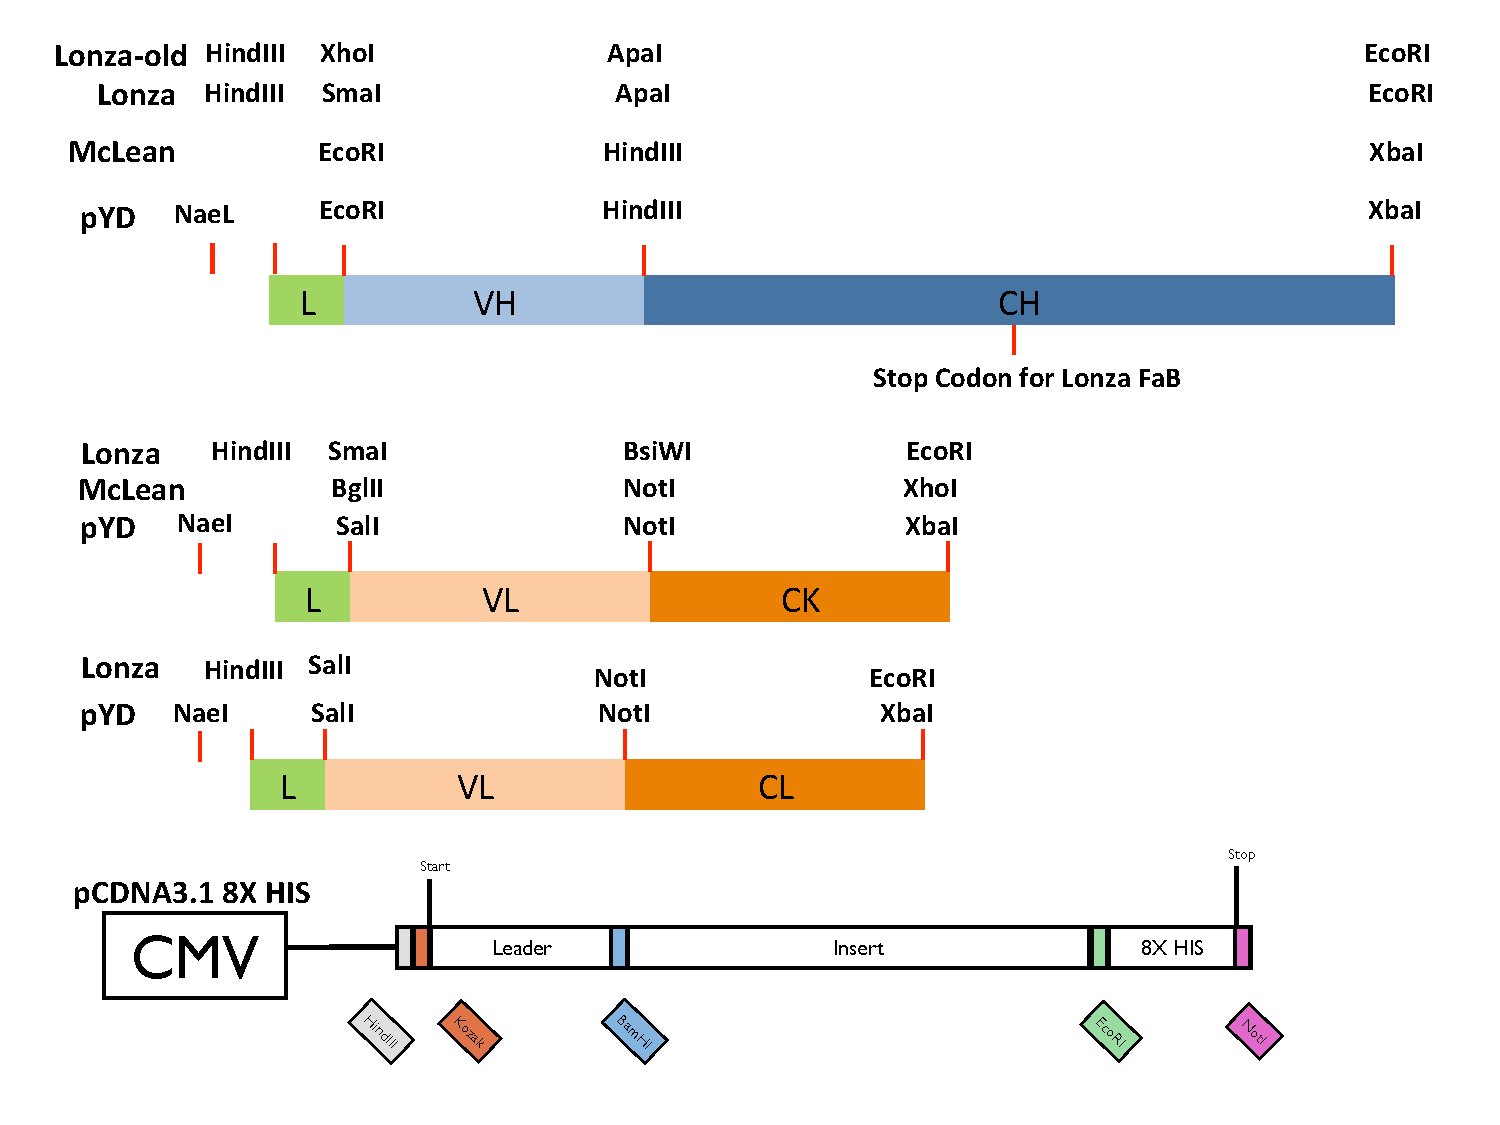
\includegraphics[scale=.85]{images/appendix/figa1.pdf}
   \caption[Restriction Maps for Common Vectors]{}
       \label{fig:figa_1}
\end{sidewaysfigure}

\clearpage

\subsection{HIV Neutralization Assay}
\textbf{Pre-Neutralization Assay} -
-Make growth media (GM) also called TZMbl media. (DMEM high glucose 1X + 110 mg/mL NaPy + 1X Pen-Strep +  10\% Heat Inactivated FBS)
-If you are testing serum, make sure to heat inactivate.

\textbf{Neutralization Assay}
Using the plate setup found in figure \ref{fig:figa_2}.
\begin{figure}[!t]
   \centering
   
\includegraphics[]{images/appendix/figa2.png}
   \caption[Neutralization Assay Plate Setup]{}
       \label{fig:figa_2}
\end{figure}

\begin{enumerate}
  \item Put 150 uL of GM into column 1
  \item Put 100 \microliter of GM in the rest of the wells
  \item Start with 7.5 $\mu$g/mL of antibody in the Dil 1 wells (Row H, columns 3-12). This well be serially diluted 3 fold and give a final dilution of 0.2 $\mu$g/mL.
  \item Fill columns 3-12, row H up to 150 \microliter with GM.
  \item Use 50 \microliter of these rows to do a serial 3-fold dilution. Discard the 50 \microliter out of the remaining row to ensure only 100 \microliter is left.
  \item Make a viral stock of 10 mL of GM to 4,000 TCID\textsubscript{50}. Viruses must be titered (see other protocols).
  \item Add 50 \microliter of 4,000 TCID\textsubscript{50} stock to columns 2-12. Make sure you don't do column 1.
  \item Cover and incubate at $37\,^{\circ}\mathrm{C}$ for 2 hours.
\end{enumerate}

While the virus and antibodies are incubating. Prepare the cells to be added at the end of the incubation.

\begin{enumerate}
  \item TZMBl cells should be confluent. Decant cell culture and wash with sterile PBS.
  \item Add 5 mL of tryspin (to T150 flask) and incubate for 1 minute.
  \item Aspirate trypsin and incubate cells at $37\,^{\circ}\mathrm{C}$ for five minutes.
  \item Add 10 mL of growth media and count cells.
  \item Dilute cells in 500 mL falcon tube to 100,000/mL with GM.
  \item If it has been two hours, take the virus and antibody plates and add 100 \microliter of cells to every well.
  \item Cover and incubate at $37\,^{\circ}\mathrm{C}$ for 48-72 hours.
  \item From every well aspirate 100 \microliter of GM.
  \item Add 100 \microliter of Bright Glow Luciferase reagent and mix 10 times in every row. Incubate for 2 minutes.
  \item Record the luminescence on a luminometer.
  \item If background is low enough, \ic can be recorded from automatic PRISM non-linear regression analysis after log\textsubscript{2} transformation of concentrations.
\end{enumerate}



\clearpage